\chapter{Análise de Concorrentes}
Auditamos soluções que existem atualmente no mercado e verificamos que das aplicações existentes há intersecções nas funções. As funções mais básicas como gerenciar itens e gerenciar listas estão presentes em todos. Mas as divergências ficam claras quando analisamos o mecanismo das aplicações, entre elas nos chamou atenção o Mealime e o Cozi Family Organizer que apesar de serem voltados para as compras focam também em outros objetivos. O Mealime com objetivo de planejamento de refeições e o Cozi Family Organizer com o objetivo de planejamento familiar, deixam a desejar nas funções relacionadas às compras.
Dos outros apps estudados verificamos também que eles não cobrem tudo o que nós nos propomos a desenvolver, especialmente em relação ao compartilhamento de listas o mecanismo difere muito entre os que possuem a função. O SoftList por exemplo permite o compartilhamento de lista mas ela não pode ser gerenciada por mais de um usuário, ou seja, compartilha-se a lista e ela é importada para o usuário que a recebeu. 
Verificando os apps mais populares da categoria constatamos que o Out Of Milk, Bring! e o OurGroceries, que são destaques na área, não se propõem a exibir análise estatística das compras do usuário e nem manter um histórico do que foi comprado.


\section{Tabela de Comparação}

	\begin{figure}[h!]
	\centering
	%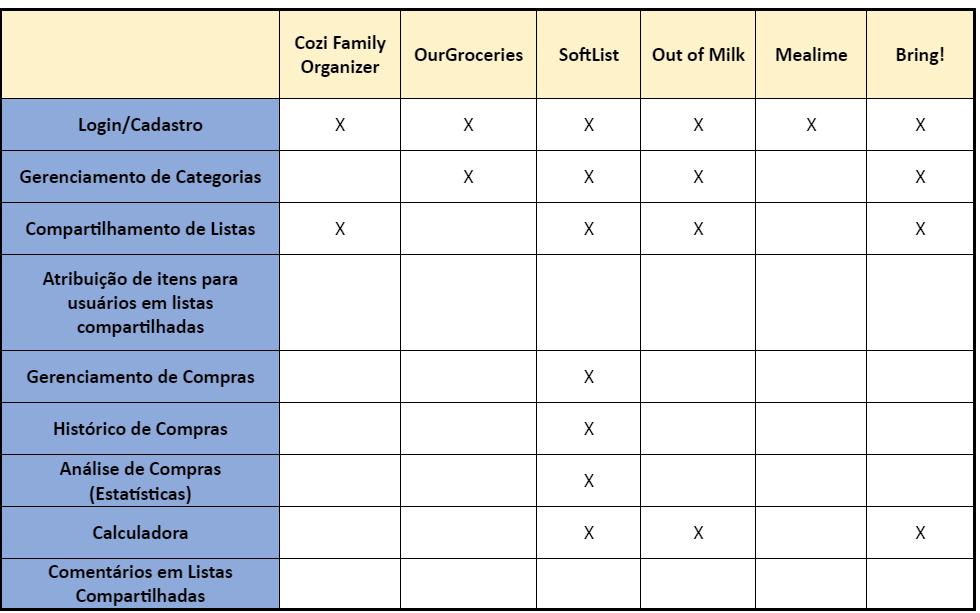
\includegraphics[scale=0.65]{./imagens/tabela_comparativa.png}
	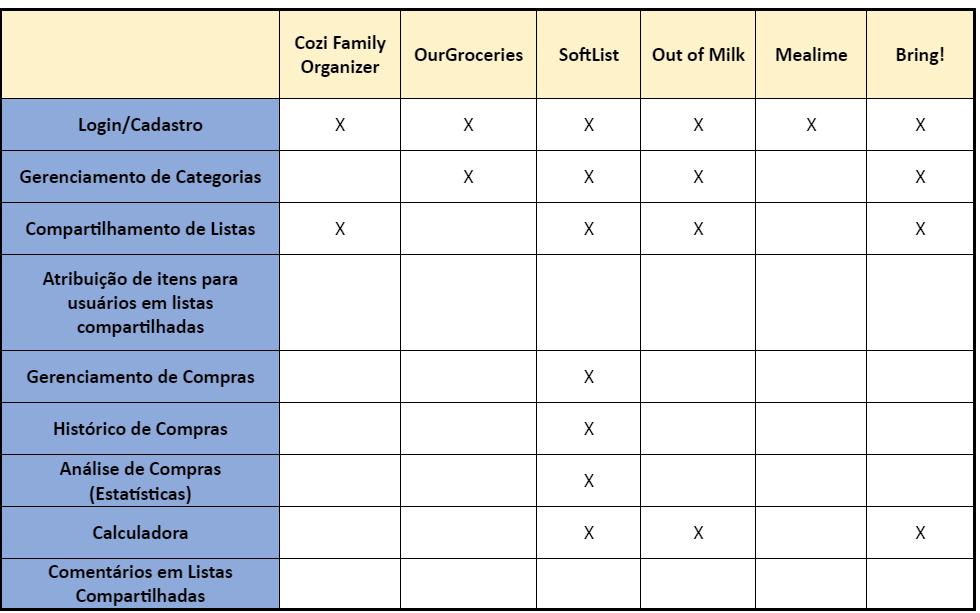
\includegraphics[width=.8\textwidth,height=\textheight,keepaspectratio]{./imagens/tabela_comparativa.png} 
	\caption{Comparativo de Concorrentes}
	\end{figure}
	